\section{Documents}\label{sec:fa_documents}

\begin{figure}[H]
  \centering
  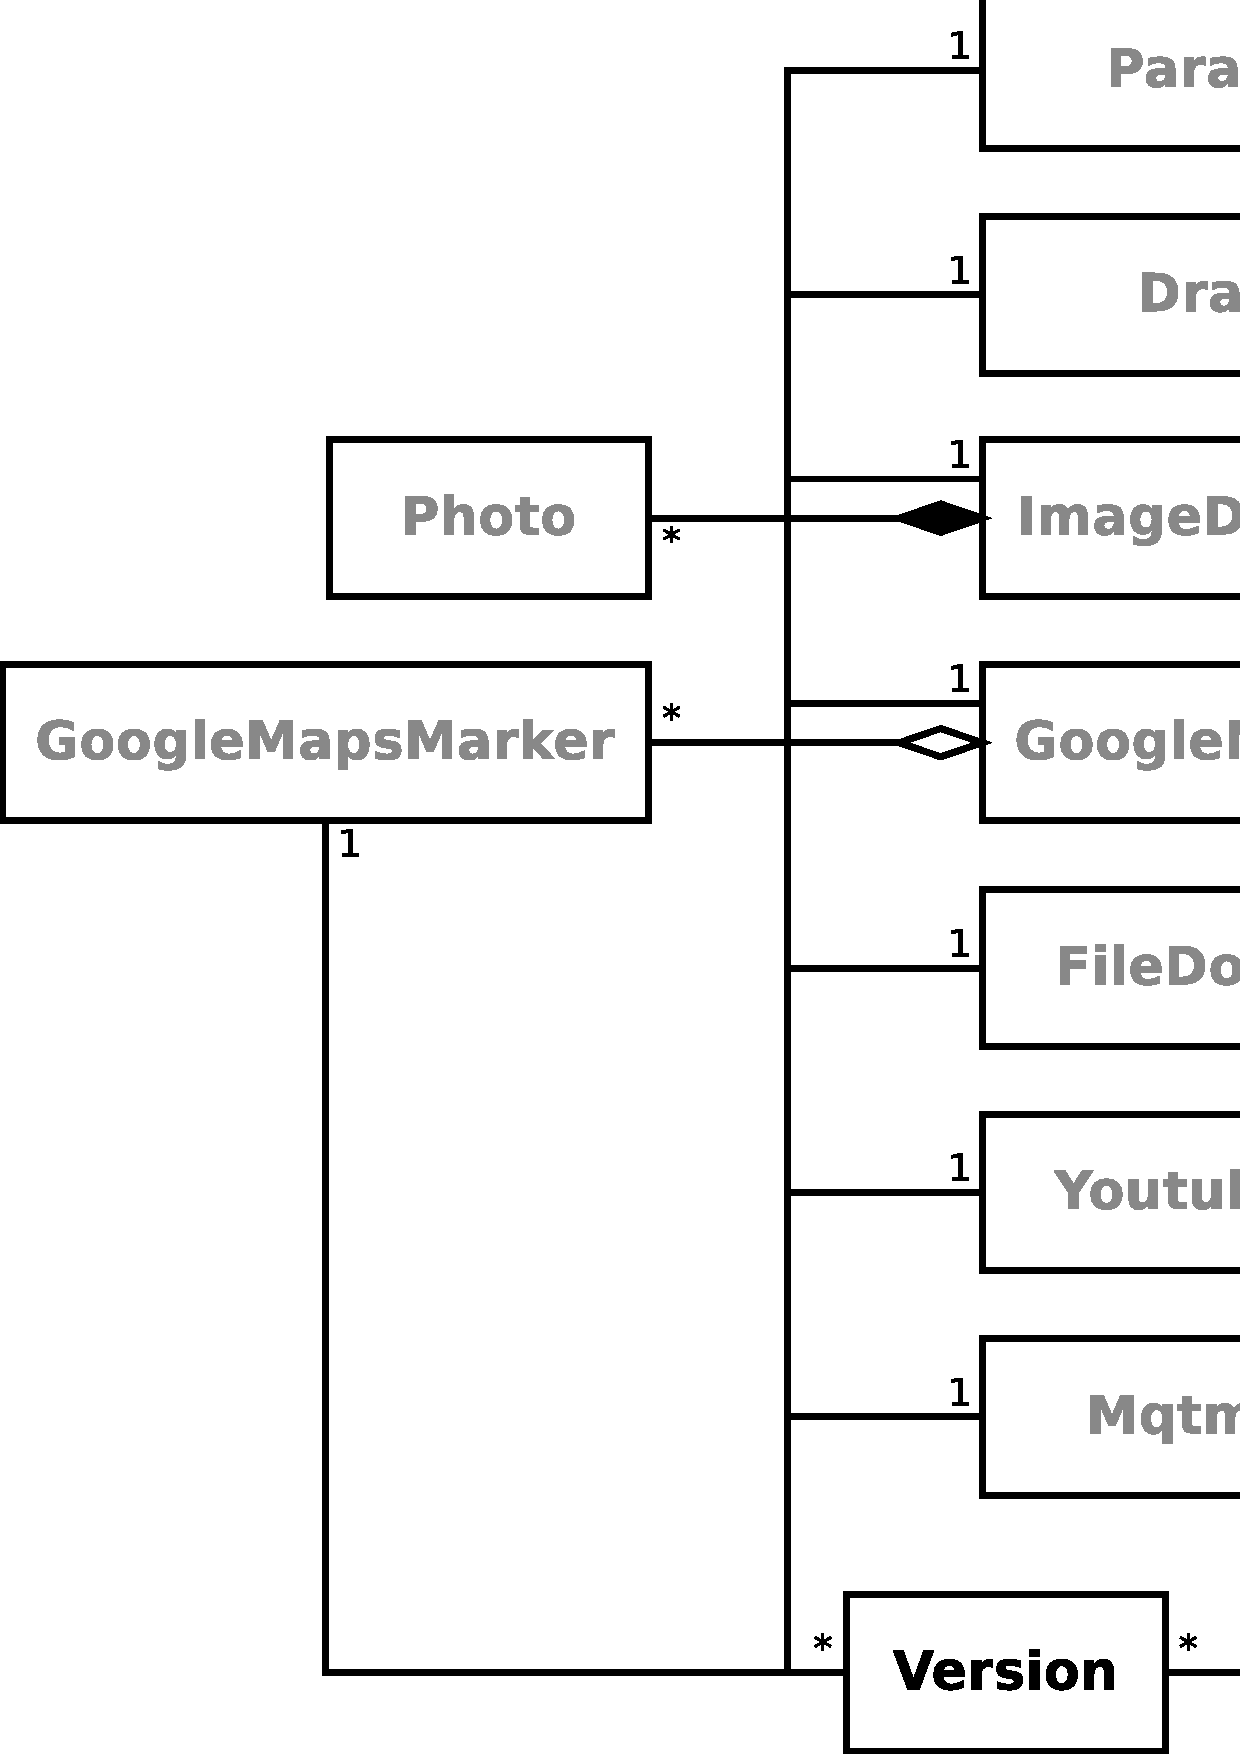
\includegraphics[width=165mm]{documents_current.pdf}
  \caption{Current Documents Model}
  \label{fig:documents_current}
\end{figure}

\subsection{Variability Requirements}\label{sec:fa_documents_variability_requirements}

\subsection{Candidate Patterns}\label{sec:fa_documents_candidate_patterns}

\subsection{Chosen Patterns \& Rationale}\label{sec:fa_documents_chosen_patterns_rationale}

The pattern used is a composite design pattern \cite{riehle_composite_patterns}, where various smaller design patterns work in tandem to create a more complex pattern.


\textbf{FIXME}

patterns used
\begin{itemize}
  \item Memento - used for versioning
  \item 
\end{itemize}

\begin{figure}[H]
  \centering
  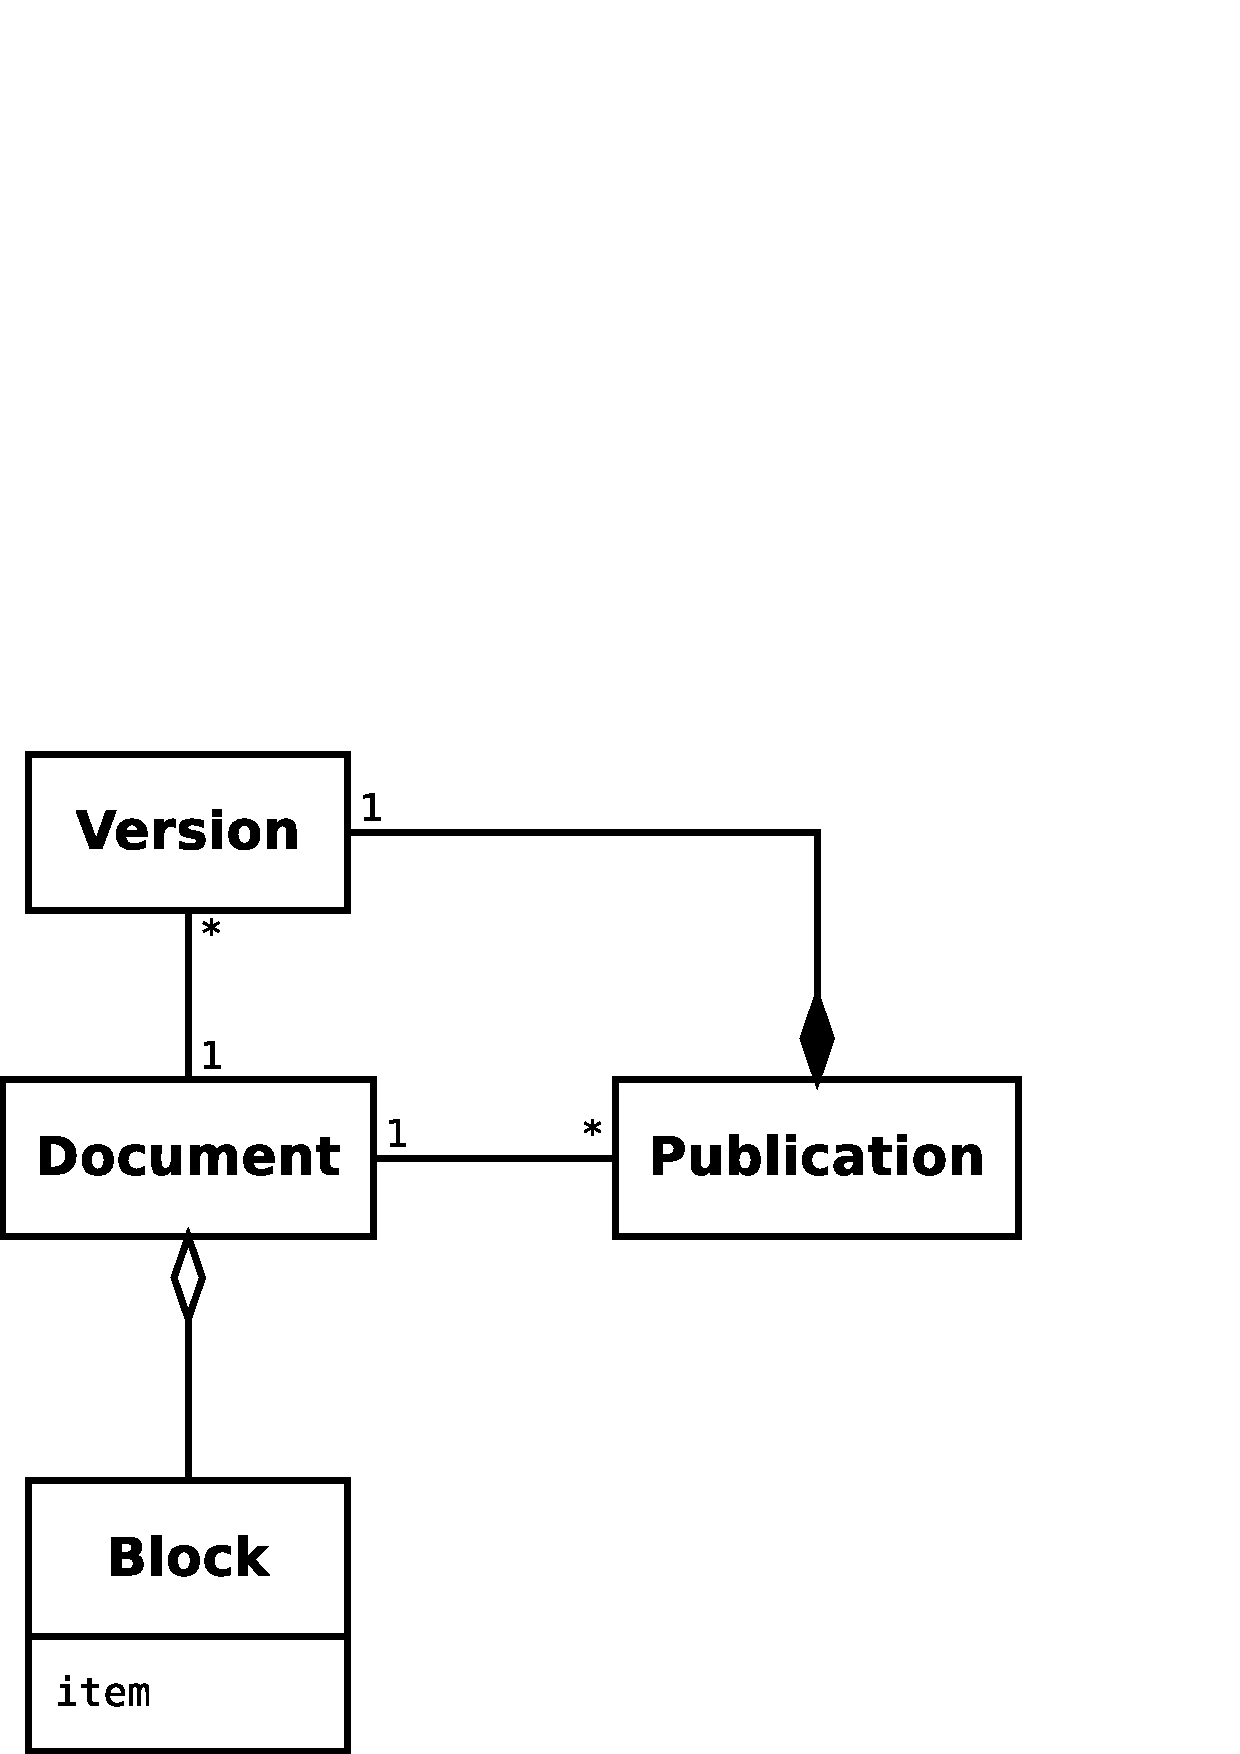
\includegraphics[width=75mm]{documents_conceptual.pdf}
  \caption{Conceptual Documents Model}
  \label{fig:documents_conceptual}
\end{figure}

\subsection{Implementation}\label{sec:fa_documents_implementation}

\subsection{Impact Analysis}\label{sec:fa_documents_impact_analysis}
